\documentclass{report}

\usepackage[brazil]{babel}
%o outro tipo de encoding geralmente usado no windows é o "ansinew"
\usepackage[utf8]{inputenc}

\usepackage{amsmath}
\usepackage{indentfirst}
\usepackage{multirow}
\usepackage{graphicx}
\usepackage{float}

\author{Eu mesmo}
\date{Hoje}
\title{Uma nova abordagem para a troca de
       lâmpadas elétricas: utilizando um banquinho}

\newcommand{\vetor}[1]{\textbf{#1}}

\begin{document}

\maketitle

\chapter{Introdução}
\label{sec:intro}

As lâmpadas elétricas são amplamente utilizadas nos dias
de hoje para a iluminação residencial.
Em geral, tais lâmpadas estão dispostas no teto dos cômodos,
longe do alcance de pessoas de estatura mediana.

% http://www.igf.min-financas.pt/inflegal/bd_igf/bd_legis_geral/leg_geral_docs/dl_650_75.htm
O pé-direito 
\footnote{pé direito se define como a distância entre o pavimento e o teto}
das construções tem valor mínimo de 2,40 metros e valor máximo de 2,70 metros.

% http://www.ibge.gov.br/home/estatistica/populacao/condicaodevida/pof/2008_2009_encaa/tabelas_pdf/tab1_1.pdf
A tabela \ref{tab:ibge} mostra alguns dos dados das estimativas populacionais das
medianas de altura e peso do povo brasileiro por sexo.

\begin{table}[!htb]
  	\centering
  	\begin{tabular}{|l|r|r|}
  	\hline
    \multirow{2}{*}{Faixa etária} & \multicolumn{2}{|c|}{Altura (cm)} \\ \cline{2-3}
                 & Masculino & Feminino \\ \hline
    18      anos & 172,6 & 161,1 \\
    19      anos & 172,0 & 161,2 \\
    20 a 24 anos & 173,0 & 161,1 \\
    25 a 29 anos & 173,0 & 160,7 \\
    30 a 35 anos & 171,6 & 160,0 \\
    \hline
    \end{tabular}
    \label{tab:ibge}
\end{table}

% Nossos estudos mostraram que um homem com o braço esticado alcança 1.35 vezes sua altura
% amostragem: 1 pessoa, eu mesmo. mascarar isso de algum jeito pra parecer mais sério
Considerando que um homem com o braço esticado alcança 1.35 vezes sua altura,
podemos dizer que um homem na faixa etária de 20 a 24 anos alcança 2.34 metros,
o que chega perto, porém ainda alguns centímetros a menos, do valor mínimo do
pé-direito residencial.
Para as mulheres, o problema é maior. Sua altura com o braço esticado alcança
2.13 metros, muito aquém do mínimo do pé-direito residencial.

O estado da arte em troca de lâmpadas nas ocasiões em que não se é possível
alcança-la meramente esticando-se o braço envolve subir nos ombros de um parceiro,
conforme a Figura \ref{fig:ombros}.

% http://loscaneros.blogspot.com.br/2012/07/quantas-pessoas-sao-nescessarias-para.html
\begin{figure}[!htb]
  \centering
  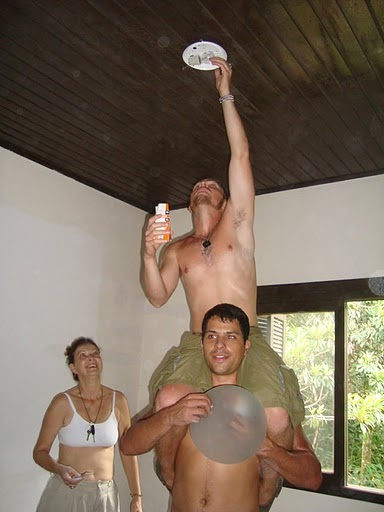
\includegraphics[width=0.5\textwidth]{ombros.jpg}
  \caption{Trocando lâmpada subindo nos ombros de um parceiro}
  \label{fig:ombros}
\end{figure}


Neste trabalho iremos apresentar uma nova abordagem
para a troca de lâmpadas elétricas:
subindo num banquinho. % hehehe

% aqui eu tenho que melhorar a introducao


\chapter{Motivação}
\label{sec:motiv}

Pessoas muito baixas não conseguem trocar lâmpadas.
O presente trabalho sugere que elas subam num
banquinho para alcançar a lâmpada.

\hfill

Como vimos na introducao (secao \ref{sec:intro}),
...

Uma fórmula qualquer: $V=R I$

$$I = \frac{V}{R}$$

$$0=1+e^{j\pi}$$

IDFT (fórmula numero \ref{eq:idft}):

\begin{equation}
\label{eq:idft}
x_n = \frac{1}{N}
\sum_{k=0}^{N-1} X_k \cdot
e^{i2\pi kn/N}
\end{equation}

Equacoes de maxwell (\ref{eq:max1} e \ref{eq:max2}).

\begin{align}
\label{eq:max1}
\nabla \cdot \vetor{E} & = \frac{\rho}{\epsilon_0} \\
\label{eq:max2}
\nabla \cdot \vetor{B} & = 0 \\
\nabla \times \vetor{E}
& = - \frac{\partial \vetor{B}}{\partial t} \\
\nabla \times \vetor{B} & =
\mu_0\vetor{J} + \mu_0 \epsilon_0
\frac{\partial \vetor{E}}{\partial t}
\end{align}

\end{document}